\documentclass{beamer}
\usetheme{Berlin}

\usepackage[T1]{fontenc}
\usepackage{textcomp}
\usepackage[utf8x]{inputenc}
\usepackage[ngerman]{babel}

\usepackage{amsmath, amsfonts, amsthm, mathtools, amssymb}

\renewcommand{\Im}{\operatorname{Im}}
\renewcommand{\Re}{\operatorname{Re}}

\newcommand{\N}{\mathbb{N}}
\newcommand{\Q}{\mathbb{Q}}
\newcommand{\R}{\mathbb{R}}
\newcommand{\Z}{\mathbb{Z}}
\newcommand{\C}{\mathbb{C}}

\newcommand{\intd}{\mathrm{d}}

\title{Die Riemannsche Zeta-Funktion}
\author{Josua Kugler}
\date{03.11.2020}

\begin{document}
%\includeonlyframes{current}
\titlepage
\section{Definition und Konvergenzgebiet}
\begin{frame}%texorpdfstring{$\zeta$}{\unichar{"03B6}}
    \begin{definition}[Riemannsche $\zeta$-Funktion]
        \[
            \zeta(s) = \sum_{n = 1}^{\infty} \frac{1}{n^s}
        \]
    \end{definition}
\end{frame}
\begin{frame}
    \begin{lemma}[Konvergenzgebiet]
        $\zeta(s)$ konvergiert normal auf der offenen Halbebene $\Re s > 1$.
    \end{lemma}
    \begin{proof}
    \[\sum_{n=1}^\infty \left|\frac{1}{n^s}\right| =  \sum_{n=1}^\infty \left|\frac{1}{e^{\log(n)\cdot \Re s}}\right| \cdot \left|\frac{1}{e^{i \cdot \log(n) \cdot \Im s}}\right| = \sum_{n=1}^\infty \frac{1}{n^{\Re s}}.\] 
    %Diese Reihe konvergiert, wie aus der reellen Analysis bekannt, für $\Re s > 1$.
    \end{proof}

\end{frame}
\section{Eulerprodukt}
\begin{frame}
    \begin{lemma}[Eulerprodukt]
        Die Riemannsche $\zeta$-Funktion lässt sich als absolut konvergentes unendliches Produkt schreiben:
    \[
        \zeta(s) = \prod_{k\in \mathbb{N}}\frac{1}{1-p_k^{-s}}.
    \]
    Insbesondere gilt also $\zeta(s) \neq 0$ für $\Re s > 1$.
    \end{lemma}
\end{frame}
\begin{frame}[t]
    \begin{proof}
    \begin{align*}%geometrische Reihe
        \visible<5->{\lim\limits_{m \to \infty}}\visible<2->{\prod_{k=1}^m} \frac{1}{1-p_k^{-s}} &= \only<5->{\lim\limits_{m \to \infty}}\only<2->{\prod_{k=1}^m} \sum_{\nu = 0}^\infty \frac{1}{p_k^{\nu s}}\\
        %Cauchyscher Multiplikationssatz
        \visible<3->{&=} \only<5->{\lim\limits_{m \to \infty}} \visible<3->{\sum_{\nu_1,\dots, \nu_m = 0}^\infty (p_1^{\nu_1}\cdots p_m^{\nu_m})^{-s}}\visible<3->{\\}
        %Eindeutigkeit der Primfaktorzerlegung
        \visible<4->{&=} \only<5->{\lim\limits_{m\to \infty}} \visible<4->{\sum_{n = p_1^{\nu_1}\cdots p_m^{\nu_m}}n^{-s}\\}
        \only<7>{\prod_{k=1}^\infty \frac{1}{1-p_k^{-s}} }\visible<6->{ &= \sum_{n=1}^\infty n^{-s}}\invisible<1->{justsomespaceforkeepingthe=}
    \end{align*}
    \end{proof}
\end{frame}
\begin{frame}
    \begin{proof}[Beweis. (Absolute Konvergenz)]
        \begin{align*}
        \sum_p \left|1 - \frac{1}{1-p^{-s}}\right| &= \sum_p \left|1 - \sum_{m=0}^\infty p^{-ms}\right|\\
        &\leq \sum_p \sum_{m=1}^\infty \left| p^{-ms}\right|\\
        &\leq \sum_{n=1}^\infty \left|n^{-s}\right|
        \end{align*}
    \end{proof}
\end{frame}
\section{Analytische Fortsetzung}
\begin{frame}
    \begin{lemma}[$\theta$-Funktion]
        Die Thetafunktion, gegeben durch
        \[
            \theta(z) = \sum_{n = -\infty}^{\infty} e^{i\pi n^2z},
        \] konvergiert für $\Im z > 0$.
    \end{lemma}
\end{frame}
\begin{frame}
    \begin{proof}
        \begin{align*}
            \visible<1->{\sum_{n = -\infty}^{\infty} \left|e^{i\pi n^2 (\Re z + i (\Im z)}\right| &= \sum_{n = -\infty}^{\infty} \left|e^{i\pi n^2 \Re z}\right|\cdot \left| e^{i \pi n^2 \cdot i (\Im z)}\right|\\}
            \visible<2->{&= \sum_{n = -\infty}^{\infty} e^{- \pi n^2 \Im z}\\}
            \visible<3->{&= \sum_{n = -N}^{N} e^{- \pi n^2 \Im z} + 2\cdot \sum_{n = N}^{\infty} e^{- \pi n^2 \Im z}\\}
            \visible<4>{&\leq \sum_{n = -N}^{N} e^{- \pi n^2 \Im z} + 2\cdot \sum_{n = N}^{\infty} \frac{1}{n^2}< \infty}
        \end{align*}
    \end{proof}
\end{frame}
\begin{frame}
    \begin{lemma}[$\theta$-Funktion]
        Die Thetafunktion, $\theta(z) = \sum_{n = -\infty}^{\infty} e^{i\pi n^2z}$, konvergiert für $\Im z > 0$.
    \end{lemma}
    \begin{behauptung}
        $\theta(z)$ erfüllt die Thetatransformationsformel ($\sqrt{\cdot}$ bezeichne den Zweig mit positivem Realteil): 
            \begin{align*}
                \theta(z) &= \theta\left(-\frac{1}{z}\right)\cdot \sqrt{\frac{i}{z}}\\
                \Leftrightarrow \theta(it) &= \theta\left(-\frac{1}{it}\right) \cdot \sqrt{\frac{i}{it}} = \theta\left(it^{-1}\right)\cdot t^{-\frac{1}{2}}.
            \end{align*}
    \end{behauptung}
\end{frame}
\begin{frame}
    \begin{lemma}
        Die Funktion 
        \[
            R_\infty(s) \coloneqq \int_1^\infty \frac{\theta(it)-1}{2} t^{s/2} \frac{\intd t}{t} = \int_1^\infty \sum_{n=1}^\infty e^{-\pi n^2 t} t^{s/2} \frac{\intd t}{t}
        \] ist ganz.
    \end{lemma}
\end{frame}
\begin{frame}
    \begin{block}{Beweis.}
        Abschätzen der Reihe ergibt
        \begin{align*}
            e^{\pi t} \cdot \sum_{n = 1}^{\infty} e^{-\pi t n^2} &= \sum_{n = 1}^{\infty} e^{-\pi t (n^2-1)}\stackrel{t \geq 1}{\leq} \sum_{n = 1}^{\infty} e^{-\pi (n^2-1)}\\
            \visible<2->{&= \sum_{n = 1}^{N} e^{-\pi (n^2-1)} + \sum_{n = N+1}^{\infty} e^{-\pi (n^2-1)}\\}
            \visible<3->{&\leq  \sum_{n = 1}^{N} e^{-\pi (n^2-1)} + \sum_{n = N+1}^{\infty} \frac{1}{n^2}\\}
            \visible<4->{&\leq B}
        \end{align*}
        \visible<5>{Also ist $\sum_{n = 1}^{\infty} e^{-\pi n^2 t} \leq B e^{-\pi t}$.}
    \end{block}
\end{frame}
\begin{frame}
    \begin{proof}
        \begin{align*}
            \int_1^\infty \sum_{n=1}^\infty e^{-\pi n^2 t} t^s \frac{\intd t}{t} &\leq B \cdot \int_1^\infty e^{-\pi t} t^{s+1} \frac{\intd t}{t^2}
            \visible<2->{\intertext{$\exists a(s):\ \forall \alpha > a: e^{-\pi \alpha} < \alpha^{-s+1}$}}
            \visible<3->{&= B \cdot \int_1^a e^{-\pi t} t^{s+1} \frac{\intd t}{t^2} + B\cdot \int_a^\infty e^{-\pi t} t^{s+1} \frac{\intd t}{t^2}\\}
            \visible<4->{&\leq B \cdot C(s) + B\cdot \int_a^\infty \frac{\intd t}{t^2}\\}
            \visible<5->{&\leq B\cdot C(s) + \frac{B}{a(s)} < \infty}
        \end{align*}
    \end{proof}
\end{frame}
\begin{frame}
    \begin{lemma}
        Die Riemannsche $\zeta$-Funktion besitzt eine analytische Fortsetzung auf $\C\setminus\{1\}$, wobei an der Stelle 1 eine einfache Polstelle vorliegt. Außerdem genügt 
        \[\xi(s) \coloneqq \pi^{-\frac{s}{2}} \Gamma\left(\frac{s}{2}\right)\zeta(s)\] der Funktionalgleichung $\xi(s) = \xi(1-s)$.
    \end{lemma}
\end{frame}
\begin{frame}
    \begin{block}{Beweis.}
        Sei $\Re s > 1$.
        \begin{align*}
            \Gamma(s) &= \int_0^\infty e^{-t} t^s \frac{\intd t}{t}&&\left|t \mapsto \pi n^2t\right.\\
            \visible<2->{&= \int_0^\infty e^{-\pi n^2t}(\pi n^2 t)^s \frac{\intd t}{t} &&\left|\cdot \pi^{-s} \cdot n^{-2s}\right.\\}
            \visible<4->{\sum_{n = 1}^{\infty}}\visible<3->{\pi^{-s} \Gamma(s)n^{-2s}&= }\only<4->{\sum_{n = 1}^{\infty}}\visible<3->{\int_0^\infty e^{-\pi n^2 t} t^s \frac{\intd t}{t}&&\left|\sum_{n = 1}^{\infty},\; s\mapsto s/2\right.\\}
            \alt<6>{\invisible<1->{\sum_{n=1}^{\infty}n^{-s}}}{\invisible<1->{\zeta(s)}}\visible<5->{\pi^{-s/2} \Gamma(s/2)\alt<6>{\zeta(s)}{\sum_{n=1}^{\infty}n^{-s}} &= \sum_{n=1}^\infty \int_0^\infty e^{-\pi n^2 t}t^{s/2} \frac{\intd t}{t}}
        \end{align*}
    \end{block}
\end{frame}
\begin{frame}
\begin{block}{Beweis.}
    \begin{align*}
        \pi^{-s/2} \Gamma(s/2)\zeta(s) &= \alt<1>{\sum_{n = 1}^{\infty} \int_0^\infty}{\int_0^\infty \sum_{n = 1}^{\infty}} e^{-\pi n^2 t}t^{s/2} \frac{\intd t}{t}\\
        \visible<3->{&= \int_0^\infty \frac{\theta(it)-1}{2} t^{s/2} \frac{\intd t}{t}\\}
        \visible<4->{&= \underbrace{\int_0^1 \frac{\theta(it)-1}{2} t^{s/2} \frac{\intd t}{t}}_{R_0(s)} + \underbrace{\int_1^\infty \frac{\theta(it)-1}{2} t^{s/2} \frac{\intd t}{t}}_{R_\infty(s)}\\}
        \visible<5->{&= R_0(s) + R_\infty(s)}
    \end{align*}
\end{block}
\end{frame}

\begin{frame}
\begin{block}{Beweis.}
    \begin{align*}
        R_0(s) &= \int_0^1 \frac{\theta(it)-1}{2} t^{s/2} \frac{\intd t}{t}\invisible<1->{\hspace*{2.2cm}}&&\left|\theta(it) = \theta(it^{-1})\cdot t^{-\frac{1}{2}}\right.\\
        \visible<2->{&= \only<3->{-}\alt<-2>{\int_0^1}{\int_1^0} \frac{\theta\left(it^{-1}\right)\cdot t^{-\frac{1}{2}}-1}{2} t^{s/2\only<4->{+1}} \frac{\intd t}{t\only<4->{^2}}&&\left|u = \frac{1}{t},\; \intd u = \frac{-1}{t^2}\intd t\right.\\}
        \visible<5->{&= \int_1^\infty \frac{\theta\left(iu\right)\cdot u^{\frac{1}{2}}-1}{2} u^{-s/2-1} \intd u\\}
        \visible<6->{&= \int_1^\infty \frac{\theta\left(it\right)\cdot t^{\frac{1}{2}}-1}{2} t^{-s/2} \frac{\intd t}{t}}
    \end{align*}
\end{block}
\end{frame}
\begin{frame}
\begin{block}{Beweis.}
    \begin{align*}
        R_0(s) &= \alt<3->{\int_1^\infty 
        \alt<3>{\frac{\theta\left(it\right)\cdot t^{\frac{1}{2}}-t^{\frac{1}{2}}}{2}\cdot t^{-s/2}}{\frac{\theta\left(it\right)-1}{2}\cdot t^{\frac{1-s}{2}}}\only<4>{}\frac{\intd t}{t} + \int_1^\infty \frac{t^{\frac{1}{2}} -1}{2} t^{-s/2} \frac{\intd t}{t}}{\int_1^\infty \frac{\theta\left(it\right)\cdot t^{\frac{1}{2}}\only<2->{-t^{\frac{1}{2}} + t^{\frac{1}{2}}}-1}{2} t^{-s/2} \frac{\intd t}{t}}\\
        \visible<5->{&= R_\infty\left(1-s\right) + \int_1^\infty \frac{1}{2}t^{\frac{1-s}{2}} \frac{\intd t}{t} - \int_1^{\infty} \frac{1}{2} t^{-s/2} \frac{\intd t}{t}\hspace*{1.4cm}\\}
        \visible<6->{&= R_\infty(1-s) + \alt<6>{\frac{1}{2}\frac{2}{1-s}}{\frac{1}{1-s}}t^{\frac{1-s}{2}}\bigg|_1^\infty + \alt<6>{\frac{1}{2}\frac{2}{s}}{\frac{1}{s}}t^{-\frac{s}{2}}\bigg|_1^\infty\\}
        \visible<8->{&= R_\infty\left(1-s\right) - \frac{1}{1-s} - \frac{1}{s}\\}
    \end{align*}
\end{block}
\end{frame}
\begin{frame}
\begin{block}{Beweis.}
    \vspace*{-0.5cm}
    \begin{align*}
        \pi^{-s/2} \Gamma(s/2)\zeta(s) &= R_\infty(s) + R_0(s)\\
        \visible<3->{\xi(s)}\visible<2->{&= R_\infty(s) + R_\infty(1-s) - \frac{1}{s} - \frac{1}{1-s}}
    \end{align*}%
    \begin{itemize}
        \item<4-> $R_\infty$ ist ganz
        \item<5-> $\xi$ ist holomorph auf $\C \setminus\{0,1\}$.
        \item<6-> $\xi$ genügt der Funktionalgleichung $\xi(s) = \xi(1-s)$
    \end{itemize}
\end{block}
\end{frame}
\begin{frame}
    \begin{block}{Beweis.}
        \begin{align*}
            \pi^{-s/2} \Gamma(s/2)\zeta(s) &= \xi(s)\\
            \visible<2->{\zeta(s) &= \frac{\pi^{s/2}}{\Gamma(s/2)}\xi(s)}
        \end{align*}
        \visible<3->{$\Gamma$ ist meromorph auf $\C$ und besitzt keine Nullstellen.\\}
        \visible<4->{$\implies$ $\frac{\pi^{s/2}}{\Gamma(s/2)}$ ist holomorph auf $\C$.\\}
        \visible<5->{$\implies$ $\frac{\pi^{s/2}}{\Gamma(s/2)}\xi(s)$ ist holomorph auf $\C\setminus\{0,1\}$.}
    \end{block}
\end{frame}
\begin{frame}
    \begin{block}{Beweis.}
        \begin{align*}
            & \lim\limits_{s \to 0} \frac{\pi^{s/2}}{\Gamma(s/2)}\bigg(\underbrace{R_\infty(s) + R_\infty(1-s) - \frac{1}{1-s}}_{\implies \text{beschränkt für } s \to 0} - \frac{1}{s}\bigg)\\
            \visible<2->{\intertext{Wegen $\lim\limits_{s \to 0} \Gamma(s/2) = \infty$ erhalten wir}}
            \visible<3->{=& 0 - \lim\limits_{s \to 0} \frac{\pi^{s/2}}{s\cdot \Gamma(s/2)} = - \lim\limits_{s \to 0} \frac{\pi^{s/2}}{2\cdot s/2\cdot \Gamma(s/2)}\\}
            \visible<4->{=& -\lim\limits_{s \to 0} \frac{\pi^{s/2}}{2\cdot \Gamma(s/2 + 1)}= -\frac{\pi^0}{2\cdot \Gamma(1)} = -\frac{1}{2}}
        \end{align*}
    \end{block}
\end{frame}
\begin{frame}
    \begin{block}{Beweis.}
        Die Funktion \[
            \frac{\pi^{s/2}}{\Gamma(s/2)}\left(R_\infty(s) + R_\infty(1-s) - \frac{1}{s} - \frac{1}{1-s}\right)
        \] ist daher
        \begin{itemize}
            \item<2-> holomorph auf $\C \setminus \{1\}$. 
            \item<3-> stimmt für $\Re s > 1$ mit $\zeta(s)$ überein
        \end{itemize}
        \visible<4->{$\implies$ stellt die gesuchte analytische Fortsetzung für die Riemannsche $\zeta$-Funktion dar!!!}
    \end{block}
\end{frame}
\begin{frame}
    \frametitle{Ergebnis}
    \begin{itemize}
        \item Für $\Re s > 1$ gilt \[\zeta(s) = \frac{\pi^{s/2}}{\Gamma(s/2)} \left(R_\infty(s) + R_\infty(1-s) - \frac{1}{s} - \frac{1}{1-s}\right).\]
        \item Damit ist eine analytische Fortsetzung nach ganz $\C\setminus\{1\}$ gefunden, wobei an der Stelle $s = 1$ eine einfache Polstelle vorliegt.
        \item Aus der Gleichung \[\xi(s) = \pi^{-s/2} \Gamma(s/2)\zeta(s) = R_\infty(s) + R_\infty(1-s) - \frac{1}{s} - \frac{1}{1-s}\] erkennt man sofort die geforderte Funktionalgleichung \[\xi(s) = \xi(1-s)\]
    \end{itemize}
\end{frame}
\section{Riemannsche Hypothese}
\begin{frame}
    \begin{hypothesis}[Riemannsche Hypothese]
        Abgesehen von den \glqq trivialen\grqq\ Nullstellen bei $s = -2n,\; n\in \N$ haben alle Nullstellen Realteil $\frac{1}{2}$.
    \end{hypothesis}
    \only<1>{
    \begin{figure}
        \begin{tikzpicture}
            \node[anchor=south west,inner sep=0] (image) at (0,0) {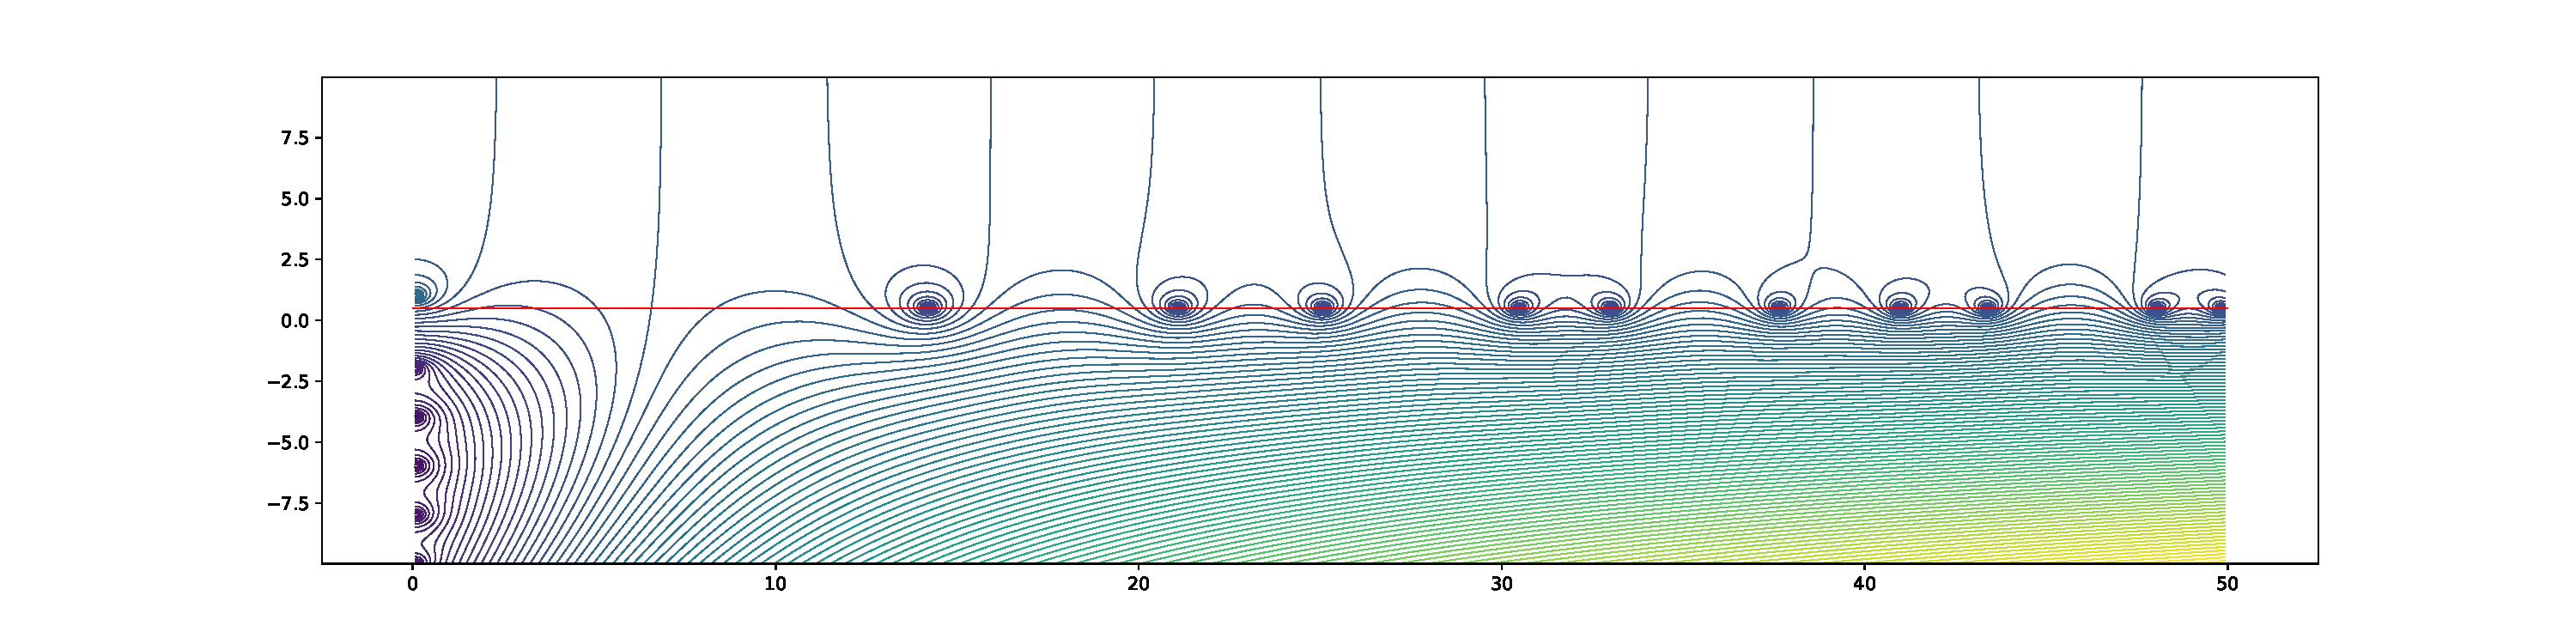
\includegraphics[width=0.8\textwidth, trim=231 46 195 44, clip]{figures/jupyter_zeros.pdf}};
            \begin{scope}[x={(image.south east)},y={(image.north west)}]
                %\draw[help lines,xstep=.1,ystep=.1] (0,0) grid (1,1);
                \foreach \y in {-10,-5,...,10} { 
                    \node [anchor=east] at (0,\y/20+0.5) {$\y$}; 
                    \draw (0,\y/20+0.5) -- (-1mm,\y/20+0.5);
                    }
                \foreach \x in {0,10,...,50} { 
                    \node [anchor=north] at (\x/50,0) {$\x$}; 
                    \draw (\x/50,0) -- (\x/50,-1mm);
                    }
                \node (ylabel) at (-.12,0.5) {$\operatorname{\Re s}$};
                \node (xlabel) at (0.5,-.25) {$\operatorname{\Im s}$};
                \draw[very thin] (0,0) rectangle (1,1);
            \end{scope}
        \end{tikzpicture}
        \caption{Absolutbetrag der $\zeta$-Funktion bei $\Re s = \frac{1}{2}$ von $\Im s = 0$ bis $\Im s = 50$}
    \end{figure}
    }
    \only<2>{
        \begin{center}
            \sagestr{output}
        \end{center}
    }
\end{frame}
\end{document}